\chapter{Initial Conditions}
\label{initialization_chap}

ARW may be run with user-defined initial conditions 
for idealized simulations, or it may be run using
interpolated data from either an external analysis or forecast for
real-data cases.  Both 2D and 3D test cases are provided for idealized
simulations.  
Several sample cases are provided for real-data simulations, which
rely on pre-processing from an external package (usually the 
WRF Preprocessing System, referred to as WPS) that converts
the large-scale GRIB-formatted data into an intermediate format suitable for ingest by the ARW's
real-data processor.

The programs that generate the specific initial conditions for the selected 
idealized or real-data case function similarly. They provide ARW with:
\begin{itemize}\setlength{\parskip}{-5pt}
\item input data that are correctly staggered for the horizontal and vertical grid;
\item hydrostatically balanced reference state and perturbation fields; and
\item metadata specifying such information as the date, grid physical characteristics,
and projection details.
\end{itemize}
\noindent Neither idealized nor real-data cases use
observations to enhance their initial conditions; however, output from 
the ARW system initial condition program is suitable as input to the WRF Variational
Data Assimilation package (see Chapter \ref{var_chap}).

\section{Initialization for Idealized Conditions}

Table \ref {ideal cases table} summarizes the names of the ARW ideal test cases that
utilize various assumptions of idealized environments.
These test cases include
a single column model (em\_scm\_xy), 
large eddy simulations (em\_les), ground fire simulations (em\_fire),
sea breezes (em\_seabreeze2d\_x), mountain waves (em\_hill2d\_x), squall lines
(em\_squall2d\_x, em\_squall2d\_y), supercell thunderstorms
(em\_quarter\_ss), gravity currents (em\_grav2d\_x), baroclinic
waves (em\_b\_wave), tropical cyclones (em\_tropical\_cyclone), 
convective-radiation equilibrium (em\_convrad), and 
global domains (em\_heldsuarez).  
A brief description of these test cases can be
found in the doc/README\.test\_cases file provided in the ARW release.
Test cases include examples of atmospheric
flow at fine scales (e.g., the LES test case has a grid-spacing of
100 meters and a time step of 1 second) and at large
scales (e.g., the Held Suarez global test case uses a grid-spacing around 600 km and
a time step of 1800 s), in addition to traditional mesoscale and
cloud-scale model simulations.  The test suite allows an ARW user to
easily reproduce these known solutions.  The test suite is also the
starting point for constructing personalized idealized flow simulations by modifying
the existing initializations that closely resemble a desired initialization.

\begin{table}
\caption{Ideal Cases. Listed are the available idealized cases for the Advanced Research WRF.}
\label{ideal cases table}
$$\vbox
{\halign{\hfil#\hfil \qquad & \hfil#\hfil \qquad & \hfil#\hfil \cr
\multispan3\hrulefill \cr
 1D             & 2D                  & 3D                    \cr
\multispan3\hrulefill \cr
em\_scm\_xy     &  em\_grav2d\_x      & em\_b\_wave           \cr
                &  em\_hill2d\_x      & em\_convrad           \cr
                &  em\_seabreeze2d\_x & em\_fire              \cr
                &  em\_squall2d\_x    & em\_heldsuarez      \cr
                &  em\_squall2d\_y    & em\_les               \cr
                &                     & em\_quarter\_ss       \cr
                &                     & em\_tropical\_cyclone \cr
\multispan3\hrulefill \cr
}}$$
\end{table}

Initial conditions for the Held-Suarez test case are analytically
defined in the initialization routines. Other than the baroclinic wave case
that utilizes a binary file providing a 2D profile specified in $[y,z]$, the remaining
idealized ARW cases use as input a 1D sounding specified as a function of
geometric height $z$. The text file defining this 1D sounding may be
directly edited by the user.  
The 1D specification of the sounding in
these test files requires surface values of pressure, potential
temperature, and water vapor mixing ratio, followed by potential
temperature, vapor mixing ratio, and horizontal wind components at some
heights above the surface.  Initialization programs for each case
assume that this moist sounding represents an atmosphere in hydrostatic
balance.

Two sets of thermodynamic fields are needed for the model--- the
reference state and the perturbation state (see Chapter
\ref{equation_chap} for discussion of the equations).  The
reference state used in idealized initializations is computed using
the input sounding from which moisture is discarded (because the
reference state is dry).  The perturbation state is computed using the full
moist input sounding.  The procedure for computing the hydrostatically-balanced 
ARW reference state and perturbation state variables from the input
sounding are as follows.  First, density and both a dry and full
hydrostatic pressure are computed from the input sounding at the input
sounding levels $z$.  This is accomplished by integrating the
hydrostatic equation vertically up the column using the surface pressure
and potential temperature as the lower boundary condition.  The
hydrostatic equation is
% 
\begin{equation} \delta_z p = - {\overline
\rho_d}^z g (1 + {\overline q_v}^z), 
\label{init_hydro}
\end{equation} 
% 
\noindent
where $\overline{\rho_d}^z$ is a two-point average between input sounding
levels, and $\delta_z p$ is the difference of the pressure between input
sounding levels, divided by the height difference.  Additionally, the
equation of state is needed to close the system:
% 
\begin{equation} \alpha_d = {1 \over \rho_d} = {R_d
\theta_m \over p_o} 
\biggl({p \over p_o}\biggr)^{-{c_v \over c_p}}, 
\label{init_state}
\end{equation}
%
\noindent
where $q_v$ and $\theta_m$ are given in the input sounding.
\eqref{init_hydro} and \eqref{init_state} are a coupled set of nonlinear
equations for $p$ and $\rho$ in the vertical integration, solved by iteration.  
Dry pressure on input sounding levels is
computed by integrating the hydrostatic relation down from the top,
excluding the vapor component.

While the full pressure (dry, plus vapor) and dry air pressure are
computed on the input sounding levels, the pressure at the model top $p_{t}$
is computed by linear interpolation in height (or possibly
extrapolation), using the height of the model top (which is an input variable).
The column mass $p_c=p_s-p_t$ is computed by interpolating the dry air
pressure to the surface, and then subtracting $p_{t}$.  Given the
column mass, the dry-air pressure at each $\eta$ level is known from the
hybrid coordinate definition \eqref{hyb_def}, and the coordinate metric 
$\mu_d$ is computed from \eqref{mu_def}.
Potential temperature from the input sounding is interpolated to
each of the model pressure levels, and the equation of state
\eqref{init_state} is used to compute the inverse density 
$\alpha_d$.  Finally, 
ARW's dry hydrostatic relation \eqref{pd_eq}
is used to compute the geopotential.  This procedure is used to compute
the reference state (based on a dry atmosphere) and the full state
(using the full moist sounding).  Perturbation variables are
computed as the difference between the full state and the reference state.  It
should also be noted that in the nonhydrostatic model integration,
inverse density $\alpha_d$ is diagnosed from the geopotential using
this dry hydrostatic relation, and pressure is diagnosed from the equation
of state using the inverse density $\alpha_d$ and the prognostic potential
temperature $\theta_m$.  Thus, ARW's prognostic variables $\mu_d$,
$\theta_m$, and $\phi$ are in exact hydrostatic balance (to machine roundoff) 
with the model equations.

\section{Initialization for Real-Data Conditions}
Initial conditions for real-data cases are pre-processed through a separate 
package called the WRF Preprocessing System (WPS, see Fig. \ref{figure:WPS_real_wrf}).  
Output from WPS is passed to the
ARW real-data pre-processor, program {\it real}, which generates initial and lateral boundary
conditions.  This section is primarily about the steps taken to build the
initial and lateral boundary conditions for a real-data case.  Even though the
WPS is outside of the ARW system, a brief description is appropriate to show the 
method for bringing raw meteorological and static terrestrial data into the model
for real-data cases.

\subsection{Use of the WRF Preprocessing System by ARW}

The WPS is a set of programs that takes
terrestrial and meteorological data (typically in GRIB format) and transforms them for input to
the ARW pre-processor program for real-data cases ({\it real}).
Figure \ref {figure:WPS_real_wrf} shows the flow of data into and out of WPS.  
The first step for the WPS is to define a physical grid (including
the projection type, location on the globe, 
number of grid points, nest locations, and grid distances) and
to interpolate static fields to the prescribed domain.
Independent of the domain configuration,
an external analysis or forecast is processed by the WPS GRIB decoder,
which diagnoses required fields and
reformats GRIB data into an internal binary format.
With a specified domain,
WPS horizontally interpolates meteorological data onto the projected domain(s). 
WPS output data (which is sent to the ARW pre-processor program for real-data cases) 
supplies a complete 3-dimensional snapshot of the atmosphere
on the selected model grid's horizontal staggering, at the selected time slices.

%
% Figure showing WPS and real and ARW
%
\begin{figure}
  \centering
  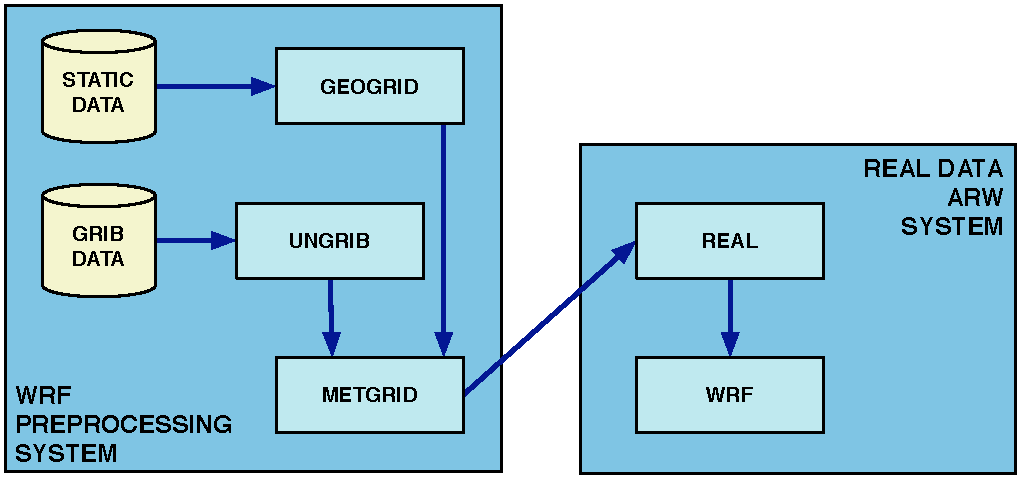
\includegraphics[width=6in]{figures/WPS_real_wrf.pdf}
  \caption{\label{figure:WPS_real_wrf}Schematic showing 
data flow and program components in WPS, and how WPS feeds initial data to ARW.
Text in the rectangular boxes indicates program names.
GEOGRID: defines the model domain and creates static files of terrestrial data.  UNGRIB:
decodes GRIB-formatted data. METGRID: interpolates meteorological data to the model domain.}
\end{figure}

Input to the ARW real-data processor from 
WPS contains surface and 3-dimensional fields
of temperature (K), relative humidity
(\%), geopotential height (m), pressure (Pa), 
and the horizontal components of wind speed (m/s, already rotated to the model 
projection).  
The 2-dimensional static terrestrial fields include
albedo, Coriolis parameters, terrain elevation, vegetation/land-use type, 
land/water mask, map scale factors, map rotation angle, soil texture category, vegetation greenness fraction, 
annual mean temperature, 
and latitude/longitude.  
After WPS processing, the 2-dimensional time-dependent fields from the external model include 
surface pressure and sea-level pressure (Pa), layers of soil temperature (K) and  soil moisture (kg/kg, 
either total moisture, or 
binned into total and liquid content), 
snow depth (m), skin temperature (K), sea surface temperature (K), and a sea ice flag.  

\subsection{Reference State}
\label{initialization_real_base_section}
Identical to idealized initializations, there is a partitioning of some 
meteorological data into reference and perturbation fields.
For real-data cases, the reference state is defined by terrain elevation and several user-definable constants:
\begin{itemize}\setlength{\parskip}{-5pt}
\item $p_{0}$ ($10^5$ Pa) reference sea level pressure; 
\item $T_{0}$ (usually 270 to 300 K) reference sea level temperature; 
\item $A$ (50 K) temperature difference between the pressure levels of $p_{0}$ and $p_{0}/e$;
\item $T_{min}$ (200 K) minimum temperature permitted; 
\item $\gamma_{strat}$ (-11 K) standard stratosphere lapse rate;
\item $p_{strat}$ (0 Pa) pressure at which stratospheric warming begins.
\end{itemize}

\noindent Using these parameters, the dry reference state surface pressure is
\begin{equation}
\bar p_{s} = p_{0}~exp\Bigg({-T_{0} \over A} + 
                     \sqrt{ {\bigg( {T_{0} \over A } \bigg)}^2 - ~
                            { 2\phi_{sfc} \over { A~R_d}} } \Bigg).
\label{init_psurf}
\end{equation}

\noindent From \eqref{init_psurf}, the 3-dimensional reference pressure (dry hydrostatic pressure $p_{d}$)
is computed as
a function of the vertical coordinate $\eta$ levels and the model top $p_{t}$:
\begin{equation}
\overline{p}_d = B(\eta) ~( \bar p_{s} - p_{t} ) +[\eta-B(\eta)](p_0-p_t) + p_{t}.
\label{init_pbar}
\end{equation}

\noindent With \eqref{init_pbar}, the reference temperature, though not permitted to get
colder than $T_{min}$, is a straight line on a skew-T plot, defined as
\begin{equation}
\overline{T}_d = \max~\bigg(~T_{min}~,~ T_0 + A~ln {\overline{p}_d \over p_0}~\bigg).
\notag
\end{equation}

\noindent For vertical locations where the $\overline{p}_d < p_{strat}$, the reference profile warms:
\begin{equation}
\overline{T}_d = T_{min} + \gamma_{strat}~ln {\overline{p}_d \over p_{strat}}.
\notag
\end{equation}

\noindent The isobaric temperature and the stratospheric correction supply a 
reasonable reference temperature up to approximately 100 Pa. 
From the reference pressure and the final reference temperature, 
the reference potential temperature is then defined as

\noindent
\begin{equation}
\overline{\theta}_d = \overline{T}_d~{\bigg( {p_0 \over \overline{p}_d } \bigg) }
^{R_d \over C_p},
\label{init_thetad}
\end{equation}

\noindent and the reciprocal of the reference density using 
\eqref{init_pbar} and \eqref{init_thetad} is given by
\begin{equation}
\overline{\alpha}_d = {1 \over \overline{\rho}_d} = {{R_d ~\overline{\theta}_d}\over p_{0} }~\bigg( 
{\overline{p}_d \over p_{0} } \bigg)^{-{C_v \over C_p}}.
\label{init_alphabar}
\end{equation}

\noindent Using \eqref{init_pbar}, the base state coordinate metric is given as
%
\begin{equation}
\bar\mu_d= {\partial \bar p_d\over\partial\eta} = B_\eta(\eta)(\bar p_s-p_t)+\bigl[1-B_\eta(\eta)\bigr](p_0-p_t).
\label{init_mubar}
\end{equation}
%
\noindent 
From \eqref{init_alphabar} and \eqref{init_mubar}, 
the reference state geopotential defined from the hydrostatic relation is
\begin{equation}
\delta_{\eta} \overline{\phi}  = -\overline{\alpha}_d~\overline{\mu}_d.
\notag
\end{equation}


\subsection{Vertical Interpolation and Extrapolation}

The ARW real-data preprocessor, {\it real}, vertically interpolates 3D input fields using functions of dry pressure.
Input data from WPS contain both a total pressure and a moisture field (typically
relative humidity).  Starting at the top of each column of input pressure data, integrated moisture
is subtracted from the pressure field, step-wise, down to the surface.  
This total dry surface pressure $p_{s}$ (diagnosed from WPS) defines the vertical coordinate metric
\begin{equation}
\mu_d = \overline{\mu}_d + \mu_d' = B_\eta(\eta)(p_s-p_t)+\bigl[1-B_\eta(\eta)\bigr](p_0-p_t).
\label{init_mutotal}
\end{equation}

\noindent
With the ARW vertical coordinate $\eta$, the model lid $p_{t}$, and the column dry
pressure known at each $(i,j,k)$ location, the 3-dimensional arrays are interpolated.

Vertical calculations are always interpolations in the free atmosphere, up to the model lid;
however, near the model surface, it is possible to have an inconsistency between the input
surface pressure (which is largely based on the input surface elevation) and the ARW surface
pressure (which could have a significantly higher-resolution topography).  These inconsistencies
may lead to an extrapolation.  The default behavior for extrapolating the horizontal winds and
the relative humidity below the known surface keeps the values constant, with zero vertical gradient.
For potential temperature, a default of 6.5 $K/km$ lapse rate is applied.
Vertical interpolation of the geopotential field is optional and is
handled separately.  Since a known lower boundary condition exists  
(the geopotential is defined as zero at the pressure at sea-level), no extrapolation is required.



\subsection{Perturbation State}

In the real-data preprocessor, first a topographically defined reference state is computed, 
then the input 3-dimensional data are vertically
interpolated in dry pressure space. With the potential temperature $\theta$ and mixing ratio
$q_v$ available on each $\eta$ level, pressure, density, and height diagnostics are
handled.
\noindent  The perturbation $\mu_d'$,
given the reference value $\overline{\mu}_d$ defined in \eqref{init_mubar} 
and the vertical coordinate metric $\mu_d$ defined in \eqref{init_mutotal},
is defined as
\begin{equation}
\mu_d'  = \mu_d - \overline{\mu}_d,
\label{init_muprime}
\end{equation}

\noindent Starting with the reference state fields 
(\ref{init_pbar}, \ref{init_alphabar}, and \ref{init_mubar}) and the perturbation (\ref{init_muprime}),
the perturbation fields for pressure and inverse density are diagnosed.
The pressure perturbation includes moisture, and is diagnosed from 
the hydrostatic equation
%
\begin{equation}
\delta_{\eta} p' = \mu'_d \bigg(1 + {\overline{q_v}^\eta} \bigg) + 
                     \overline{q_v}^\eta~\overline \mu_d,
%\label{init_pprime}
\notag
\end{equation}
%
\noindent 
which is
integrated down from 
the model top (where $p'= 0$) to recover $p'$.
The total dry inverse density is given as
\begin{equation}
\alpha_d = {R_d \over p_{0} } ~ \theta_m~ 
                                        \bigg( {{p'_d + \overline {p}_d} \over p_{0} } \bigg )^{-{C_v \over C_p}},
\notag
\end{equation}

\noindent which defines the perturbation field for inverse density

\begin{equation}
\alpha'_d = \alpha_d - \overline{\alpha}_d.
\notag
\end{equation}

\noindent 
The perturbation geopotential 
is diagnosed from the hydrostatic relation
\begin{equation}
\delta_{\eta} \phi'  = - \big ( {\mu}_d \alpha'_d + \mu'_d
\overline{\alpha}_d \big )
\notag
\end{equation}
%
by upward integration, using the terrain elevation as the lower boundary condition.

\subsection{Generating Lateral Boundary Data}

This section deals with generating the separate lateral boundary condition file used
exclusively for real-data cases.  For information
on which lateral boundary options are available for both idealized and real-data
cases, see Chapter \eqref{lbc_chap}.

For real-data cases, the specified 
lateral boundary condition for the coarse grid is supplied by an external file that is
generated by program {\it real}.
This file contains 
records for the fields $u$, $v$, $\theta$, $q_v$, $\phi'$, and $\mu'_d$ that are used by ARW to
constrain the lateral boundaries (other fields are in the boundary file, but are not used).   
The lateral boundary file holds one less time period than was processed by WPS.
Each of these variables has both
a valid value at the initial time of the lateral boundary time, and a tendency term to get to the 
next boundary time period.  For example, assuming a 3-hourly availability of data from WPS,
the first time period of the lateral boundary file
for $u$ would contain data for both coupled $u$ (map scale factor and $\mu_d$ interpolated to 
the variable's 
staggering) at the 0 h time

\begin{equation}
%U_{0h} = {{\mu_u~u}\over{m_u}} \bigg | _{0h}
U_{0h} = {{\overline{\mu_d}^x u}\over{\overline{m}^x}} \bigg | _{0h},
\notag
\end{equation}
\noindent and a tendency value defined as
\begin{equation}
U_t = { U_{3h} - U_{0h} \over 3h},
\notag
\end{equation}

\noindent which would take a grid point from the initial value to the value at the 3-hour simulation time. 
The horizontal momentum fields are coupled both with  $\mu_d$ and the inverse map factor.  The 
other 3-dimensional fields ($\theta$, $q_v$, and $\phi'$) are coupled only with $\mu_d$.
The $\mu'_d$ lateral boundary field is not coupled.

Each lateral boundary field
is defined along the four sides of the 
rectangular grid (loosely referred to as the north, south, east, and west sides).  
Boundary values and tendencies for vertical velocity and the non-vapor moisture species are included
in the external lateral boundary file, but act as
place-holders for the nested boundary data for the fine grids.
The width of the lateral
boundary zone along each of the four sides is user-selectable at run-time
(as shown in Fig. \ref{figure:spec}).

\subsection{Masking of Surface Fields}

Some of the meteorological and static fields are masked.  A masked field is one in which
values are typically defined only over water (e.g., sea surface temperature) or defined
only over land (e.g., soil temperature).
The need to match all of the masked fields consistently to each other requires additional steps
for real-data cases due to the masked data's presumed use in various physics packages in the soil, 
at the surface, and in the boundary layer.
If the land/water
mask for a location is flagged as a water point, then vegetation and soil categories must also
recognize the location as the special water flag for each of their respective categorical indices.  
Similarly, if the land/water mask is flagged as a land point, vegetation and soil
categories must be assigned to one of the available land indices.

Values for soil temperature and soil moisture come from WPS, and are on the 
native levels originally defined for those variables
by an external model.  WPS does not vertically interpolate
soil data.  While it is typical to attempt to match the ARW soil scheme with
the incoming data, that is not a requirement.  Pre-processor {\it real} will vertically interpolate 
(linear in depth below the ground) from the incoming levels to the requested soil layers to be
used within the model.

\section{Digital Filtering Initialization}

ARW provides a digital filtering initialization (DFI) to 
remove noise, which results from imbalances between mass and wind fields, 
from the model initial state. DFI is applied to output from the {\it real} 
preprocessor before the model simulation begins. If data assimilation is 
performed using WRF-Var, DFI is applied to analysis produced by the 
WRF-Var system, rather than the output of program {\it real}.

Under the assumption that any noise is of 
higher frequency than meteorologically significant modes, DFI attempts to 
remove this noise by filtering all oscillations above a specified cutoff 
frequency. Accordingly, filters in the ARW DFI are low-pass digital 
filters, which are applied to time-series of model fields. The {\it initialized} 
model state is the output of the filter at some prescribed time, 
(e.g., the analysis time). Time series of model states are generated through 
combinations of integration types that may include adiabatic, backward integration and diabatic, and/or forward 
integration in the model, along with the chosen DFI scheme (which determines the 
specific combination of integration). Three DFI schemes are available: 
digital filter launch (DFL; \cite{lynchhuang94}), diabatic DFI (DDFI; \cite{huanglynch93}), 
and twice DFI (TDFI; \cite{lynchhuang94}).

\subsection{Filter Design}

In ARW DFI, either nonrecursive (i.e., finite impulse response) digital 
filters or a recursive (i.e., infinite impulse response) digital filter may 
be used. Coefficients for the nonrecursive digital filters may be 
computed according to one of two methods, while coefficients for the 
recursive filter are computed according to a single method.

A general nonrecursive digital filter is of the form

\begin{equation}
y_n = \sum_{k=-N}^{N} h_k x_{n-k},
\label{fir_filter}
\end{equation}

\noindent
where $y_n$ is the output of the filter at time $n$, the $h_k$ are the 
coefficients of the filter, and $\{ \ldots , x_{n-1}, x_n, x_{n+1}, \ldots \}$ 
is the sequence of input values to be filtered; such a filter is said to have 
span $2N+1$. 

One method for deriving the coefficients of a nonrecursive digital filter is 
the windowed-sinc method, described in the context of DFI by \cite{lynchhuang92}. 
In the ARW DFI, either the Lanczos, Hamming, Blackman, Kaiser, Potter, or 
Dolph-Chebyshev windows may be used; the Dolph-Chebyshev window is described 
by \cite{lynch97}. However, when a filter with a shorter span is desired, 
another nonrecursive digital filter - the Dolph filter - may be used. \cite{lynch97} 
describes the construction of the Dolph filter, and demonstrates that this 
filter has properties nearly indistinguishable from those of an optimal filter, 
which minimizes the maximum difference between a filter's transfer function 
and an ideal transfer function in the pass and stop bands. 

The only recursive filter in ARW DFI is the second-order Quick-Start 
filter of \cite{lynchhuang94}. In general, a recursive digital filter that 
depends only on past and present values of input, and on past values of 
output, is of the form

\begin{equation}
y_n = \sum_{k=0}^{N} h_k x_{n-k} + \sum_{k=1}^{N} b_k y_{n-k}.
\end{equation}

\noindent
However, this form is inconvenient when inputs to the filter consist of 
model states, and storing many such states should be avoided. \cite{lynchhuang94} 
show how this type of recursive filter can be reformulated to the same 
form as a nonrecursive filter, and thus, the second-order 
Quick-Start filter follows the same form as (\ref{fir_filter}).

\subsection{DFI Schemes}

ARW supports three different DFI schemes, illustrated graphically in 
Fig. \ref{figure:dfi_types}. The DFL scheme produces an initialized model 
state valid some time after the model analysis time, while the DDFI and TDFI 
schemes produce initialized states valid at the analysis time.

%
% Figure showing available DFI schemes
%
\begin{figure}
  \centering
  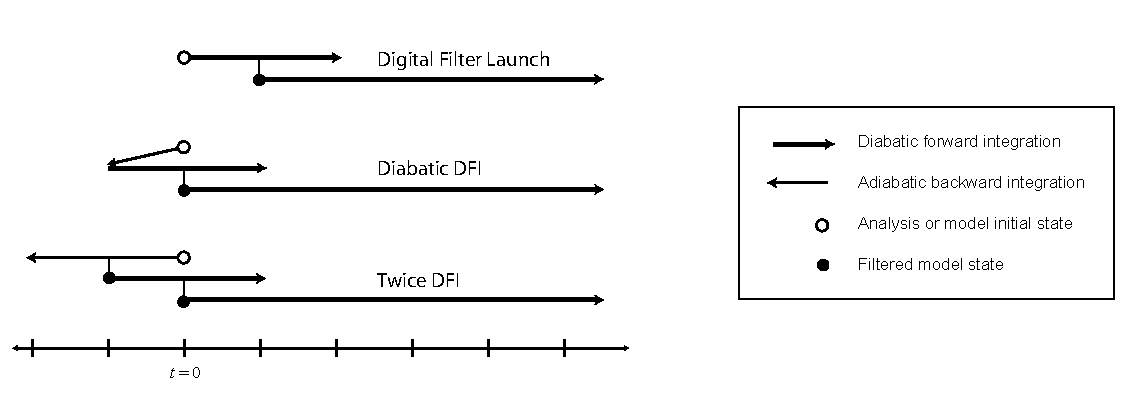
\includegraphics[width=6.5in]{figures/dfi_schemes.pdf}
  \caption{\label{figure:dfi_types}An illustration showing the three available DFI schemes: digital filter 
  launch, diabatic digital filter initialization, and twice digital filter initialization.}
\end{figure}

\subsubsection{DFL}

In the DFL scheme, forward integration with full model physics and diffusion 
begins at the initial time and continues for $2N$ time steps, during which 
time a filtered model state valid $N$ time steps beyond the analysis time is 
computed as in (\ref{fir_filter}). Then, the initialized simulation is 
launched from the midpoint of the filtering period. For any model state ${\bf X}$, 
let $\left[ {\bf X} \right]_n^D$ give the model state after diabatically 
integrating $n$ time steps forward in time; we emphasize that the superscript 
$D$ indicates diabatic integration, in contrast to adiabatic integration. 
Then, the DFL scheme is expressed as

\begin{equation}
{\bf X}_{ini} = \sum_{n=0}^{2N} h_n \left[ {\bf X}_{ana} \right]_n^D,
\end{equation}

\noindent
where ${\bf X}_{ini}$ is the initialized model state, ${\bf X}_{ana}$ is the 
model analysis or model initial state generated by the {\it real} preprocessor, 
and $h_n$ represents filter coefficients.

\subsubsection{DDFI}

To produce an initialized state valid at the model analysis time, the DDFI 
scheme begins with an adiabatic, backward integration for $N$ time steps, 
followed by a diabatic, forward integration for $2N$ time steps, during which 
filtering takes place. This filtered state is valid at the model analysis time. 
Letting $\left[ {\bf X}_{ana} \right]_{-n}^A$ denote the model state after 
adiabatic, backward integration for $n$ time steps from the model analysis or 
model initial state, ${\bf X}_{ana}$, the DDFI scheme is expressed as

\begin{equation}
{\bf X}_{ini} = \sum_{n=0}^{2N} h_n \left[    \left[ {\bf X}_{ana} \right]_{-n}^A   \right]_n^D,
\end{equation}

\noindent
where ${\bf X}_{ini}$ is the initialized model state valid at the model analysis time.

\subsubsection{TDFI}

The TDFI scheme involves two applications of the digital filter. Adiabatic, 
backward integration proceeds from the model initial time for $2N$ time steps, 
during which a filter is applied. The filtered state is valid at time $-N \Delta t$. 
From this filtered state, a forward, diabatic integration is launched. The 
second integration proceeds for $2N$ time steps, during which a second filter 
is applied, giving a filtered model state valid at this model analysis time. 
The TDFI scheme is expressed as

\begin{equation}
{\bf X}_{ini} = \sum_{n=0}^{2N} h_n \left[    \sum_{n'=0}^{2N} h_{n'} \left[ {\bf X}_{ana} \right]_{-n}^A \right]_n^D.
\end{equation}

\subsection{Backward Integration}

To diabatically integrate backward in time, it suffices to disable all 
diabatic processes and to negate the model time step $\Delta t$ as well as 
the sign of the horizontal velocity $U$ in the odd-order advection 
operators of Section \ref{advection}, which become

\begin{align}
\hbox{3}^{rd} \hbox{ order:} ~~~~ & 
(\overline{q}^{x_{adv}})_{i-1/2} = 
(\overline{q}^{x_{adv}})_{i-1/2}^{4^{th}} 
\notag
\\
&~~~~~~~~~~~~~~~~~~~~
- \hbox{sign}(U){1 \over 12} \bigl[
(q_{i+1}-q_{i-2}) - 3(q_i - q_{i-1}) \bigr]
\notag
\\
\hbox{5}^{th} \hbox{ order:} ~~~~ & 
(\overline{q}^{x_{adv}})_{i-1/2} = 
(\overline{q}^{x_{adv}})_{i-1/2}^{6^{th}} 
\notag
\\
&~~~~~~~~~~~~~~~~~~~~
+ \hbox{sign}(U){1 \over 60} \bigl[
(q_{i+2}-q_{i-3}) - 5(q_{i+1} - q_{i-2}) 
+ 10(q_i - q_{i-1})
\bigr].
\notag
\end{align}

When specified boundary conditions are used, as in Section \ref{lbc_spec}, 
the model boundaries before the model initial time are taken to be the same 
as those valid at the model initial time. We note that, with a negated time 
step, the linear ramping functions $F_1$ and $F_2$ of (\ref{lbc_relax}) 
change sign, and, consequently, so does the sign of the tendency for a 
prognostic variable $\psi$.
